\documentclass[12pt, oneside, a4paper]{book}
\usepackage{setspace}
\usepackage{arabtex}
\usepackage{utf8} 
\usepackage{hyperref} 
\usepackage{graphicx}
\usepackage{subcaption}
\usepackage{geometry}
\usepackage{lipsum}
\usepackage{listings}
\usepackage{xcolor}
\usepackage{enumitem}
\usepackage{titlesec}
\usepackage{xparse}
\usepackage{verbatim}
\usepackage{float}
\usepackage{array}
\usepackage{ragged2e}
\usepackage{tabularx}
\usepackage{verbatimbox}
\usepackage{fancyhdr}
\usepackage{tocbibind}
\usepackage[toc]{appendix}
\usepackage[final]{pdfpages}

%
 \geometry{a4paper,inner=1.25in,outer=1.25in,top=1in,bottom=1in,footskip=15mm,headsep=30mm, headheight=-3mm}
% \renewcommand{\chaptermark}[1]{\markboth{\textit{\uppercase{chapter \thechapter. #1}}}{}}

\titlespacing*{\chapter}{0pt}{-\baselineskip}{1em}
\pagestyle{fancy} % Turn on the style
\renewcommand{\headrulewidth}{0pt}

\fancyhf{} % Start with clearing everything in the header and footer
\rhead{
	{\tiny 
		\RL{المملكة العربية السعودية} \\
		\RL{وزارة التعليم العالي} \\
		\RL{جامعة الأميرة نورة بنت عبد الرحمن} \\
		\RL{كلية علوم الحاسب والمعلومات} \\
		\RL{مشروع تخرج ١}}
}
\chead{
\includegraphics[width=.1\linewidth]{img/pnu.png}}
\lhead{
	{\tiny Kingdom of Saudi Arabia \\
		Ministry of Higher Education \\
		Princess Nourah bint Abdulrahman University \\
		Faculty of Computer \& Informaion Science \\
		Graduation Project I}
}
\cfoot{\thepage}%

\fancypagestyle{plain}
{
	\rhead{
		{\tiny \RL{المملكة العربية السعودية} \\
			\RL{وزارة التعليم العالي} \\
			\RL{جامعة الأميرة نورة بنت عبد الرحمن} \\
			\RL{كلية علوم الحاسب والمعلومات} \\
			\RL{مشروع تخرج ١}}
	}
	\chead{
\includegraphics[width=.1\linewidth]{img/pnu.png}}
	\lhead{
		{\tiny Kingdom of Saudi Arabia \\
			Ministry of Higher Education \\
			Princess Nourah bint Abdulrahman University \\
			Faculty of Computer \& Informaion Science \\
			Graduation Project I}
	}
	\cfoot{\thepage}%
}
\fancypagestyle{firstpage}
{
	\rhead{
		{\tiny \RL{المملكة العربية السعودية} \\
		\RL{وزارة التعليم العالي} \\
		\RL{جامعة الأميرة نورة بنت عبد الرحمن} \\
		\RL{كلية علوم الحاسب والمعلومات} \\
		\RL{مشروع تخرج ١}}
	}
	\chead{
\includegraphics[width=.1\linewidth]{img/pnu.png}}
	\lhead{
		{\tiny Kingdom of Saudi Arabia \\
		Ministry of Higher Education \\
		Princess Nourah bint Abdulrahman University \\
		Faculty of Computer \& Informaion Science \\
		Graduation Project I}
	}
}
\usepackage{xpatch}
\xapptocmd{\titlepage}{\thispagestyle{firstpage}}{}{}

\newcommand{\mychapter}[1]{\newpage%
	\thispagestyle{empty}
	\topskip0pt%
	\vspace*{\fill}%
	\addtocounter{chapter}{1}%
	\begin{center}%
		\textbf{\Large{\color{chapter}{CHAPTER NO. \thechapter \\ \uppercase{#1}}}}%
	\end{center}%
	\vspace*{\fill}%
	\addtocounter{chapter}{-1}
	\newpage%
	\chapter{#1}
}

\definecolor{chapter}{HTML}{773344}
\definecolor{section}{HTML}{f03a47}
\definecolor{sub}{HTML}{065143}
\definecolor{ssub}{HTML}{4381c1}
\definecolor{bold}{HTML}{cc3f0c}


\definecolor{lightgray}{HTML}{eeeeee}
\definecolor{darkgray}{rgb}{.4,.4,.4}
\definecolor{purple}{rgb}{0.65, 0.12, 0.82}
\definecolor{green}{rgb}{0,0.6,0}


\titleformat{\chapter}
{\color{chapter}\normalfont\Large\bfseries}
{\color{chapter}\thechapter}{1em}{}

\titleformat{\section}
{\color{section}\normalfont\fontsize{12}{16}\bfseries}
{\color{section}\thesection}{1em}{}

\titleformat{\subsection}
{\color{sub}\normalfont\fontsize{12}{14}\bfseries}
{\color{sub}\thesubsection}{1em}{}

\titleformat{\subsubsection}
{\color{ssub}\normalfont\fontsize{12}{13}\bfseries}
{\color{ssub}\thesubsubsection}{1em}{}


\newcommand{\code}[1]{{\color{red}\colorbox{lightgray}{#1}}}
\newcommand\boldcolor[1]{\textcolor{bold}{\textbf{#1}}}
\newcommand\Includegraphics[2][]{\addvbuffer[3pt 0pt]{\includegraphics[#1]{#2}}}

\lstset{frame=tb,
	language=Java,
	aboveskip=3mm,
	belowskip=3mm,
	showstringspaces=false,
	columns=flexible,
	basicstyle={\small\ttfamily},
	numbers=none,
	numberstyle=\tiny\color{gray},
	keywordstyle=\color{blue},
	commentstyle=\color{dkgreen},
	stringstyle=\color{mauve},
	breaklines=true,
	breakatwhitespace=true,
	tabsize=3
}
\setcounter{secnumdepth}{3}
\setcounter{tocdepth}{3}
\hypersetup{
	colorlinks,
	citecolor=[rgb]{0,0.5,0.5},
	filecolor=[rgb]{0,0.5,0.5},
	linkcolor=[rgb]{0,0.5,0.5},
	urlcolor=[rgb]{0,0.5,0.5}
}


\begin{document}
	\setcode{utf8}
	
	\pagenumbering{gobble}

	\begin{titlepage}
	%=========================
	\begin{center}
		\hspace{0pt}\\
		\vspace{4cm}
		{\scalebox{1}{\large\bfseries\color{section}\uppercase{Online Home Automation Control System}}}\\			
			\vspace{2cm}
			By: \\
			\begin{table}[H]
				\begin{center}
					\begin{tabular}{rl}		
						\texttt{436200058} & Abeer Ahmed Ezzat 
						\\
						\texttt{436200063} & Doha Nidal AlZouhbi
						\\
						\texttt{437004005} & Mona Saud AlKhathlan  
						\\
						\texttt{437004100} & Nouf Abdullah AlDajani 
						\\	
						\texttt{437004875} & Reem Ali AlGhamdi
						\\
						\texttt{436006939} & Sarah Khalid AlHussain 
					\end{tabular}
				\end{center}
			\end{table}
			
			Supervised By: \\
			\Large{Dr. Aeer Mahmoud}\\
			
			
			
			% ----------------------------------------------------------------
			\vfill \normalsize
			A Graduation Project Report Submitted to \\
			College of Computer and Information Sciences at PNU \\
			in Partial Fulfillment of the Requirements for the \\
			Degree of \\
			Bachelor of Science \\
			in \\
			Computer Sciences \\[5ex]
			CCIS, PNU \\
			Riyadh, KSA \\
			1440 - 1441H \\
			% ----------------------------------------------------------------
		\end{center}
	\end{titlepage}
	\newpage

	\addcontentsline{toc}{chapter}{\nameref{sec:ack}}
	\chapter*{Acknowledgment}
	\label{sec:ack}
	\paragraph{} First and foremost, we thank Allah the Almighty for always blessing us and for helping us complete this project on time. We would like to express our special thanks of gratitude to our project supervisor Dr. Abeer Mahmoud for her continuous support, motivation, and for always commenting on our best qualities and enhancing them. Without her direction and proper guidance, this project would not have succeeded. We thank her for her unwavering support. Not to forget our loving families and supporting friends for helping us sticking to the schedule. Last but not least we want to thank anyone who has helped us by providing information, insight, comments or facilities that we needed to complete our project. Our heartfelt thanks to everyone we have mentioned.



	\pagenumbering{roman}

	%\addcontentsline{toc}{chapter}{Table of Contents}
	\tableofcontents
	\newpage	
	\doublespacing
	\newpage
	
	\listoftables
	\newpage
	
	\listoffigures
	\newpage
	
	\addcontentsline{toc}{chapter}{\nameref{sec:sym}}
	\chapter*{List of Symbols \& Abbreviations}
	\label{sec:sym}
	\def\arraystretch{1.5}
	\begin{table}[H]
		\caption{List of Symbols \& Abbreviations}
		\begin{center}
			\begin{tabularx}{\linewidth}{|c|X|}\hline
				
				\boldcolor{Symbols \& Abbreviations} & \boldcolor{Meaning} \\\hline
				UI & User Interface\\\hline
				API & Application programming Interface\\\hline
				GPIO & General Purpose Input Output\\\hline
				IDE & Integrated Development Environment \\\hline
				IoT & Internet of Things \\\hline
				LED & Light Emitting Diode\\\hline
				REST & Representational State Transfer\\\hline
				SDLC & Software Development Life Cycle\\\hline
				SQL & Structured Query Language\\\hline
				Raspberry Pi & low cost, credit-card sized computer\cite{raspberry}. \\\hline
				Linear solenoid &  type of electromagnetic actuator that converts an electrical signal into a magnetic field producing a linear motion\cite{linear}.\\\hline
			\end{tabularx}
		\end{center}
	\end{table}
	\newpage
	\addcontentsline{toc}{chapter}{\nameref{sec:kw}}
	\chapter*{Keywords}
	\label{sec:kw}
	\def\arraystretch{1.5}
	\begin{table}[H]
		\caption{Keywords}
		\begin{center}
			\begin{tabularx}{\linewidth}{|c|X|}\hline		
				\boldcolor{Keyword} & \boldcolor{Definition} \\\hline
				Raspberry Pi & low cost, credit-card sized computer\cite{raspberry}. \\\hline
				Linear solenoid &  type of electromagnetic actuator that converts an electrical signal into a magnetic field producing a linear motion\cite{linear}.\\\hline				
			\end{tabularx}
		\end{center}
	\end{table}
	\newpage
	\addcontentsline{toc}{chapter}{\nameref{sec:intro}}
	\chapter*{Abstract}
		\label{sec:intro}
		\paragraph{} The aim for this project is to control light buttons, air conditioners, television or other home appliance regardless of the person's location. The methodology is simple: an android app will send controlling requests to a web server. Raspberry Pi will be getting all the new requests from the server, processing it accordingly and controlling the hardware components connected to it. Such a system will allow someone in the United States to turn the lights in their house in Saudi Arabia on. However, an active connection to the internet must be present all the time. 
		
	

	\mychapter{Introduction}
		\pagenumbering{arabic}
		\section{Problem statement \& Significance}
		\paragraph{}With the recent very rapid progress in technology and automation, there has
		become a need for remote control of almost all possible aspects of living. Especially
		the house appliances that surround us, because of how easy they make the modern
		human’s life and how much they allow him to focus on his main work 
		instead of doing these remotely controlled tasks himself. 
		\paragraph{}Some examples we have already encountered and used in our daily lives include using apps to control a cleaning robot or adjust the heating in the house or switch the house lights on or off. For the latter, there have been many applications that can do that. However, they all work in a small set of devices and sensors. It is necessary for such applications to exist, as a service like this would be important for many people. An example is working moms who are outside the house and want to switch the lights on at a certain time to wake their children up. Another example is pet owners who need to have UV lights switched on for their pets at certain times of the day but can’t do so immediately and so on. 
		\paragraph{}However, the main challenge in creating a device to solve this problem is where the idea of IoT (Internet of Things) comes in; learning how to control this device through the Internet from afar, rather than being controlled by infrared rays locally as is the case with most similar applications. 
		\section{Proposed Solution}
		\paragraph{}The created app should enable the user, by clicking on the appropriate buttons, to control a physical apparatus that needs to be pushed to work, such as lights buttons. This will be done by designing and creating an Android application, then using a small laptop, called Raspberry Pi, to control a small piece that will be pushed forward (on command) to switch the light on or off, the API is a web application hosted on a server.
		
		\subsection{Aims}
			\paragraph{}At the end of this project, we intend to achieve the following aims:
			\begin{itemize}
	 			\item Learn how to design a mobile application using previously learned and new knowledge
				\item Learn how to invoke a web API and use it in our application
				\item Learn Python programming language to control Raspberry Pi
				\item Learn Flask web micro-framework
			\end{itemize}
		\subsection{Goals}
			\paragraph{} At the end of this project, we expect to deliver:
			\begin{itemize}
				\item An Android application with a user friendly, simple, clear interface with buttons to control a LED and linear solenoid.
				\item A physical apparatus composed of the Raspberry Pi connected to and controlling the piece.
				\item A web application following REST architecture, managing user  requests and Raspberry Pi's responses.
			\end{itemize}
		\section{Project Domain \& Limitation}
			\subsection{Domain}
				\paragraph{} Although the application will be available for all kinds of users to use, we expect that the ones who would make the most use of it would be employees who have long working hours and would need to be able to remotely control appliances in their homes, especially lights.
				\paragraph{} The critical piece in all of this application would be the linear solenoid actuator i.e. the small electrically controlled piece that would be placed very close to the light switch and would, on command, spring forward to press on the switch to turn it on or off. 
			\subsection{Limitation}
			\paragraph{} The main limitation of the application is that it will be able to control only a limited type of home appliance. Mainly things than could be pushed to work. A much more advanced application would be able to control most of the other appliances, such as controlling an Air conditioner if the owner is outside, or a timer controlled coffee maker.
			
		\section{Gantt Chart}
		\begin{figure}[H]
  			\caption{Gantt Chart}
			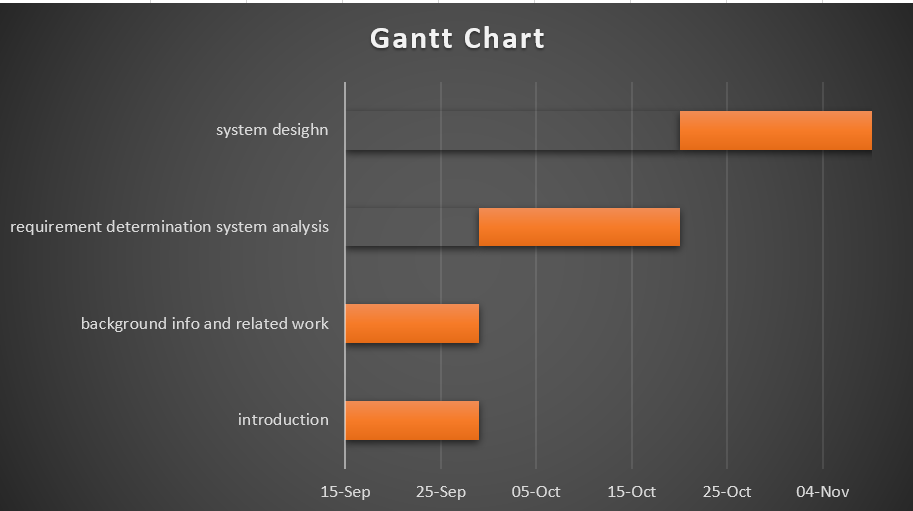
\includegraphics[width=\linewidth]{img/gantt_chart.png}
		\end{figure}
		\newpage	
		\mychapter{Background Information \& Related Work}
			\section{Background Information}
			\subsection{IoT}
			\paragraph{}The internet of things (IoT) constitutes one of the most important technological
			development in the last decade. The IoT term was coined by Kevin n 1999\cite{iot_1}. IoT
			means a “world-wide network of interconnected objects uniquely addressable, based
			on standard communication protocols”\cite{iot_2}. in a somewhat simplified manner, we
			can describe IoT is the ability to connecting as many things by the internet without
			direct human intervention by using technologies such as cloud computing, Radio
			Frequency Identification (RFID), wireless communication, sensors, Internet
			protocol, ultra-low-power processors and others\cite{iot_3}.
			\subsubsection{IoT Architecture}
			\paragraph{} IoT Architecture includes three layers Perception layer, Network layer, and
			Application layer each of them has its own functionality.
			\begin{itemize}
				\item \boldcolor{Perception layer:} is responsible to perceive and identifying objects or things in the
				environment.
				\item \boldcolor{Network layer:} is responsible for receiving and transmitting data between layers.
				\item \boldcolor{Application layer:} is the interface for all previous Layers used to processed and
				transported data to provide services to the users\cite{iot_4}.
			\end{itemize}
			\subsubsection{IoT Applications}
			\paragraph{}The Applications of the IoT are diversified and can be classified into three main
			categories industry, environment, and society.
			\begin{itemize}
			\item \boldcolor{Industry:} The importance of the industry domain can be seen in transportation,
			aviation, and automotive (e.g.Tesla automobile ).
			\item \boldcolor{Environment:} The society Domain focused on telecommunication, smart building,
			home, and medical technology (e.g.connected door locks, Closed-loop (automated)
			insulin delivery).
			\item \boldcolor{Society:} The environment Domain focused on recycling, disaster alerting,
			environmental monitoring (e.g.Forest Fire Detection, Air Pollution)\cite{iot_5}.
			\end{itemize}
			\subsection{Hardware}
				\begin{itemize}
				\item \boldcolor{Raspberry Pi:} a small general purpose computer. All hardware components will be connected to it. An active connection to the internet is needed for it to fetch data from the server\cite{raspberry}. %insert figure here% 
				\item \boldcolor{Ubuntu Web Server:} hosts the web application. Digital Ocean severs\cite{digital_ocean} were chosen for this project.
				
				\item \boldcolor{LED:} since the hardware components controlled depends heavily on the user needs, this project main aim will be controlling a small LED. LED stands for light-emitting diode\cite{led}. Basically a small light source. %insert figure here% %
				\item \boldcolor{Linear Solenoid:} once the LED works, linear solenoid will be installed for demonstrating the idea\cite{linear}. It is a small component that generates a linear motion. It will be used to press in anything, such as lights, TV remote, and coffee machine. %insert figure here%
				\end{itemize}
				
			\subsection{Programming Languages \& Frameworks}
				\begin{itemize}
					
					\item \boldcolor{Python:} raspberry pi can be controlled by either c++ or python. Python was chosen because a REST API can be made using it fast.
		 				\begin{itemize}
		 					\item \textbf{GPIO:} a library for controlling any hardware component connected to the GPIO pins\cite{gpio}.
		 					\item \textbf{Flask:} a lightweight framework to build web applications.
						\end{itemize}
					\item \boldcolor{Java:} mobile application are made in a native way with either swift or java.
						\begin{itemize}
							\item \textbf{Android:} a framework for making android apps.
							\item \textbf{Retrofit:} type-safe HTTP client for Android and Java\cite{retro}. It will be used to send and receive commands and status from the web server.
							
						\end{itemize}
					\item \boldcolor{PostgreSQL:} an open-source RDBMS\cite{postgres}. It will be installed on the server.
				\end{itemize}
			
			\subsection{SDLC Model}
			\paragraph{} Incremental model will be used in this project. This model is a process of software development where requirements are broken down into multiple standalone modules of software development cycle. Incremental development is done in steps from analysis design, implementation, testing / verification, maintenance\cite{sdlc}. The reason this model was chosen is the pieces will be installed, tested and connected to the system gradually. First a LED, then a linear solenoid and so on.
			
			
		\newpage	
		\section{Related Work}
		\subsection{Insteon - Insteon Hub}
		\begin{figure}[H]
  			\caption{Related Work: Insteon}
			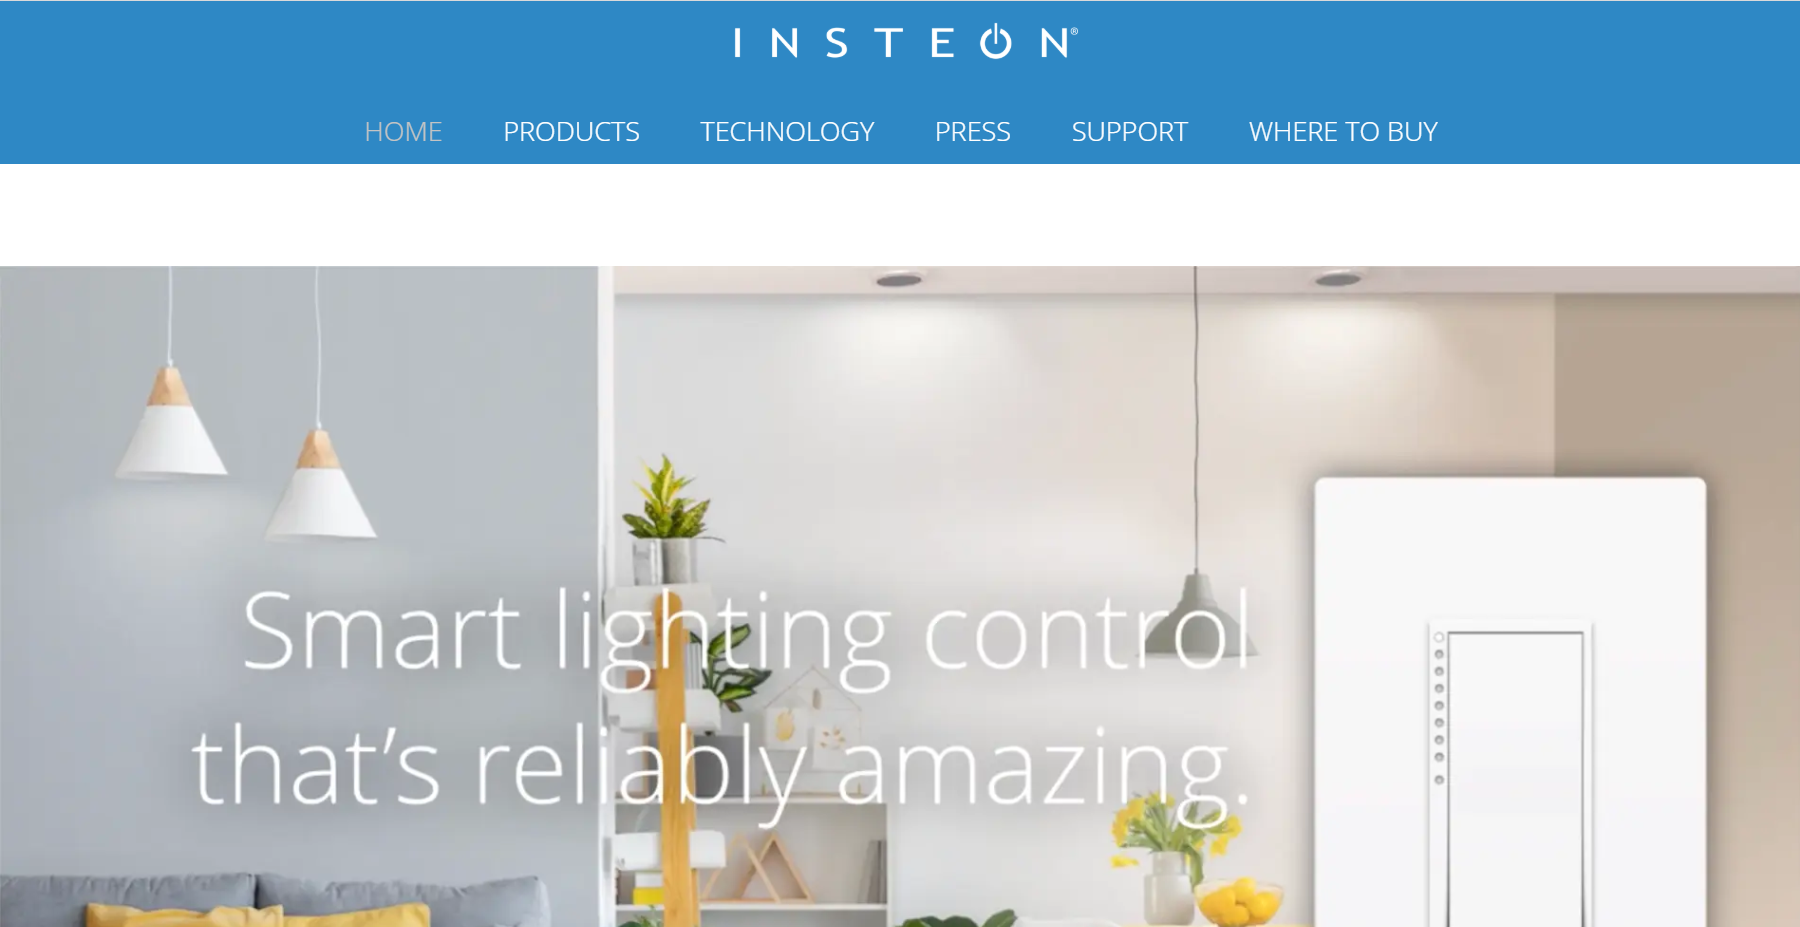
\includegraphics[width=\linewidth]{img/insteon.png}
		\end{figure}
		\paragraph{}Insteon Hub is a simple and straightforward system that connects you to your home from any smartphone or tablet, anywhere in the world. Control Insteon light bulbs, wall switches, outlets, and thermostats at home or remotely and receive instant email or push notification alerts from motion, door and window, water leak, and smoke sensors while you’re away\cite{insteon}.
		\begin{itemize}
		\item \boldcolor{Advantage:}
			\begin{enumerate}
				\item Control Multiple Devices Simultaneously with a Basic Scene.
				\item Create Schedules to Turn Your Lights On and Off at Specific Times.
				\item Automatically Turn Lights On and Off with Sensors.
				\item Monitor Your Home with Email or Push Notification Alerts.
			\end{enumerate}
		\item \boldcolor{Disadvantage:} 
			\begin{enumerate}
				\item Hub setup takes a couple of minutes and a few moments per light switch, sensor.
				\item Its need to connect it to power and your home's internet router so if the internet die all devices need to start over again. 
				\item fixed the hub take more cost than its original price.
				\item There is no database save/restore. You have to recreate all the devices, scenes, schedules if its replaced.
			\end{enumerate}
		\end{itemize}
		\newpage	
		\subsection{Wink - Wink Hub 2}
		\begin{figure}[H]
  			\caption{Related Work: Wink}
  			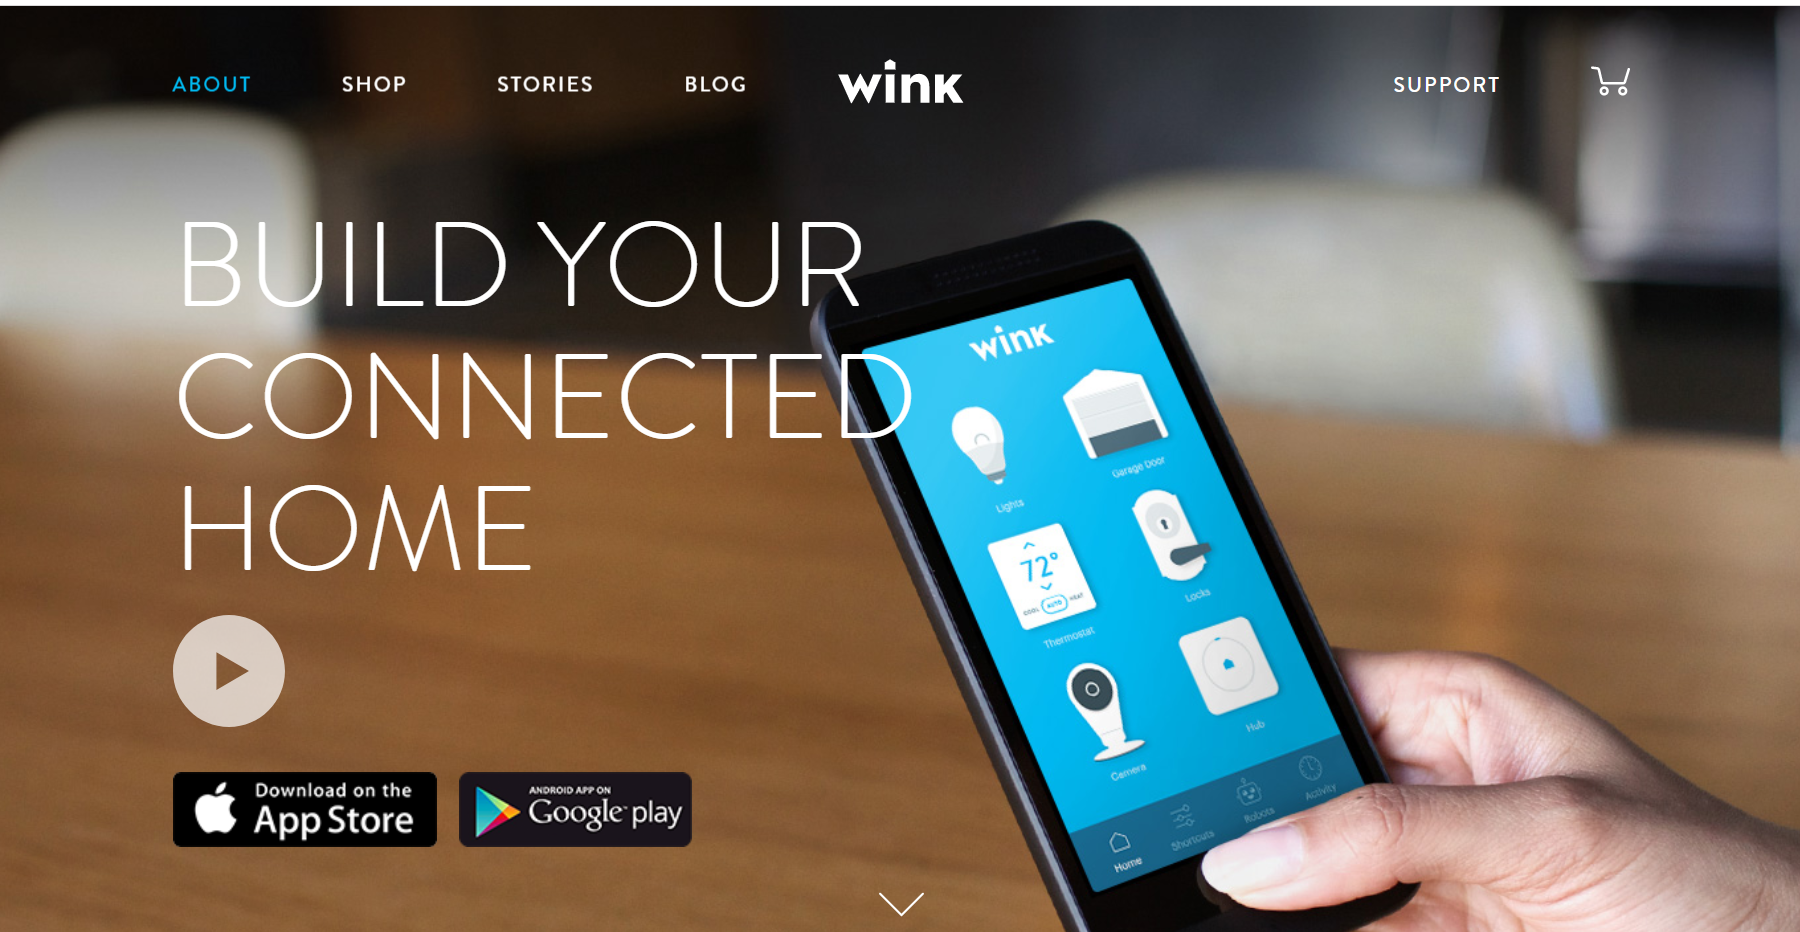
\includegraphics[width=\linewidth]{img/wink.png}
		\end{figure}
		\paragraph{}Wink Hub 2 is the world’s first smart home hub created for the mainstream consumer. With industry-leading smart home protocol support, enhanced connectivity features, and a sleek design, Wink Hub 2 brings hundreds of products from best-in-class brands together for a simple, intuitive experience\cite{wink}.
		
		\begin{itemize}
			\item \boldcolor{Advantage:}
			\begin{enumerate}
				\item Support Different platforms such as iOS or Android.
				\item Once you've created an account, Wink has the ability to recognize the products within Wink Bright, guide you through a few simple steps, and then you're ready to go.
				\item Wink works with Cortana Microsoft’s voice assistant and Amazon Alexa.
				\item One Important features in wink, its can see what you’re spending even before the bill arrives.
			\end{enumerate}
			\item \boldcolor{Disadvantage:} 
			\begin{enumerate}
				\item One major problem with the Wink 2 hub is that the device sometimes loses connectivity and must be reset in order for it to connect again.
				\item Wink app doesn't always let you access other devices' full features.
				\item High price.
				\item Takes 14 days to arrive.
			\end{enumerate}
		\end{itemize}
		\newpage
		\subsection{Samsung – Smart Things Hub}
		\begin{figure}[H]
  			\caption{Related Work: Samsung}
			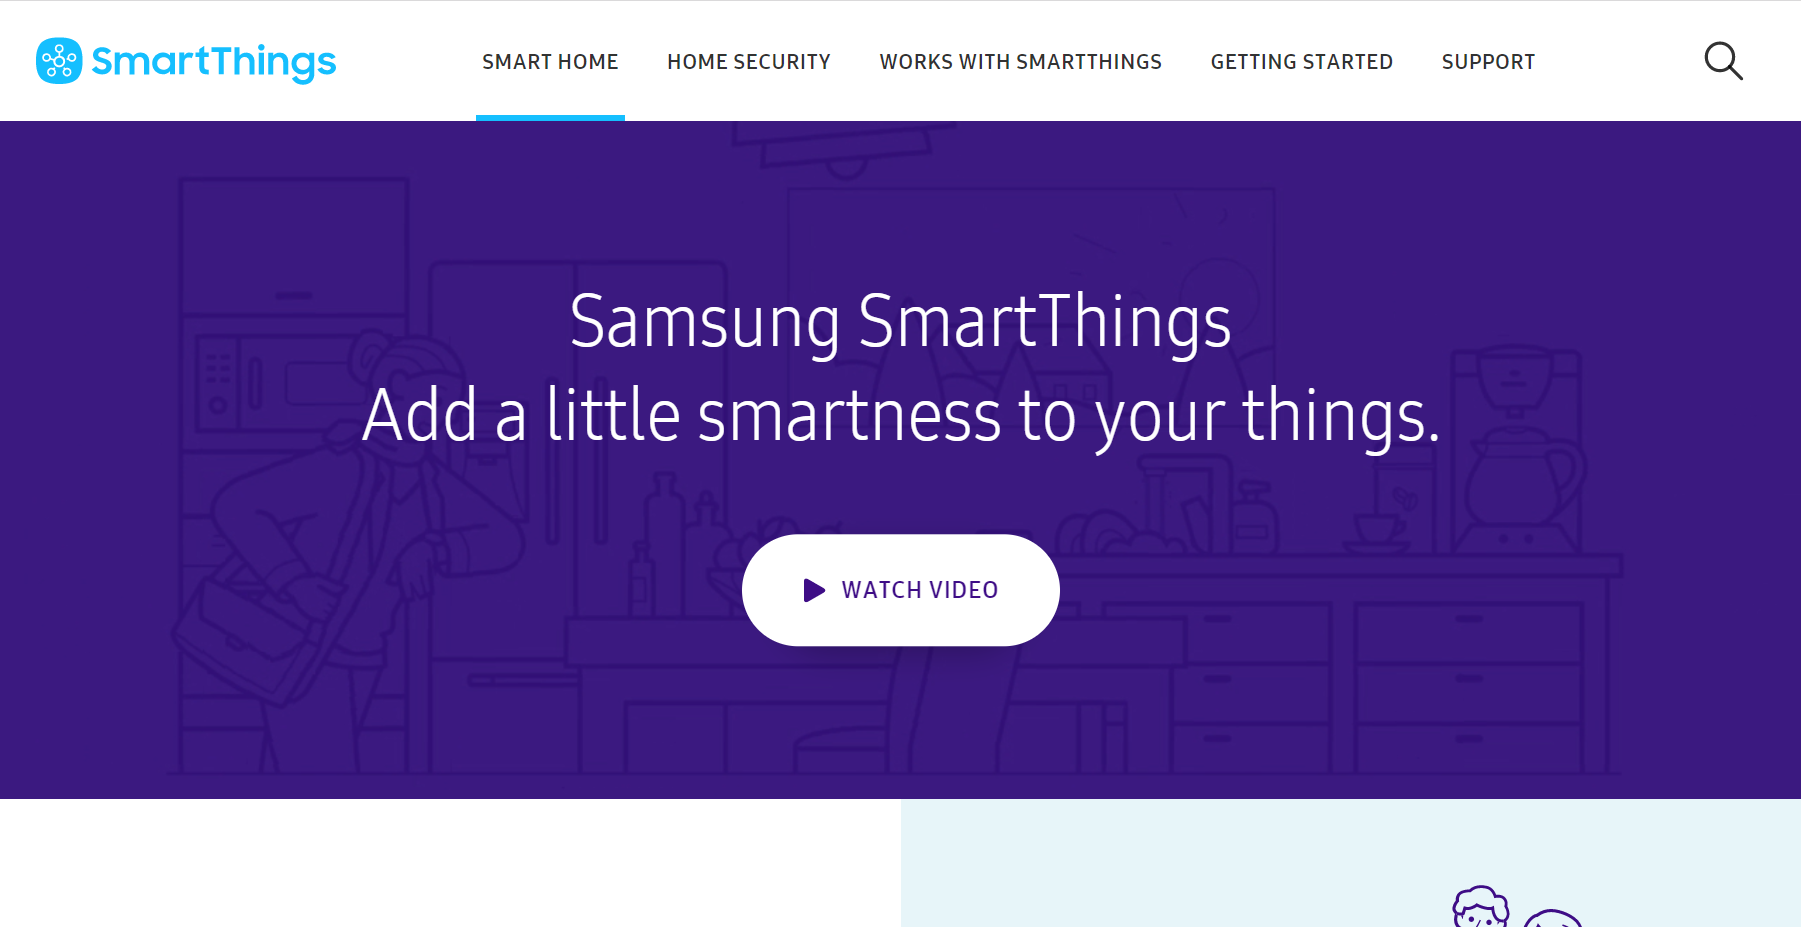
\includegraphics[width=\linewidth]{img/samsung.png}
		\end{figure}
		\paragraph{}Smart things hub Connect wirelessly with a wide range of smart devices and make them work together\cite{samsung}.
		\begin{itemize}
			\item \boldcolor{Advantage:}
			\begin{enumerate}
				\item Monitor and control connected devices in your home using a single SmartThings app for iPhone or Android.
				\item Manage connected devices in your home with SmartThings Routines for Good Morning, Goodbye, Good Night, and more.
				\item Receive alerts from connected devices when there’s unexpected activity in your home.
				
			\end{enumerate}
			\item \boldcolor{Disadvantage:} 
			\begin{enumerate}
				\item Some compatible components may not work as efficiently or smoothly as you want them to, which may be inconvenient.
				\item Some users report it stops working at times.
				\item Difficult to upgrade from older hub.
				\item In US Only.
			\end{enumerate}
		\end{itemize}
		\section{Proposed \& Similar System Comparison}
			\def\arraystretch{1.5}
			\begin{table}[H]
				\caption{Proposed \& Similar System Comparison}
			\begin{center}
			\begin{tabularx}{1\linewidth}{|m{2.2cm}*4{|X}|}\hline
					
					& \boldcolor{Raspberry Pi} & \boldcolor{Insteon} & \boldcolor{Wink hub 2} & \boldcolor{Samsung (smart things)}  \\\hline
					
					\boldcolor{design} &
						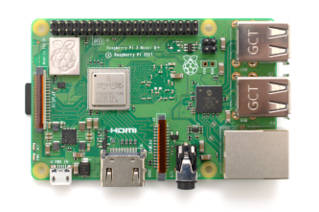
\includegraphics[width=\linewidth]{img/raspberry.png} &
						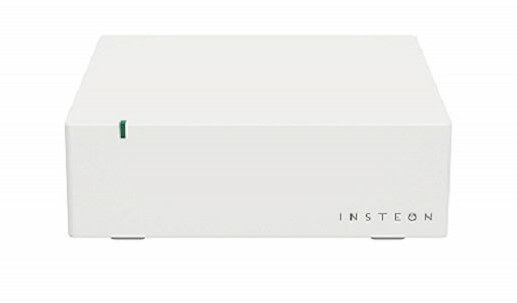
\includegraphics[width=\linewidth]{img/insteon_hw.png} & 
						\Includegraphics[width=\linewidth]{img/wink_hw.png} &
						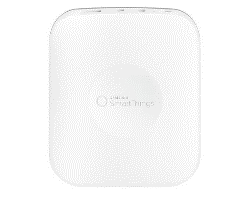
\includegraphics[width=\linewidth]{img/samsung_hw.png}
					 \\\hline
					\boldcolor{Works With Wi-Fi} & yes & yes & yes & yes  \\\hline

					\boldcolor{Price} & 25\$, parts are very cheap & 80\$, expensive parts & 99\$, very expensive parts & 70\$, expensive parts \\\hline
					
					\boldcolor{Installation \& Configuration Difficulty} & hard to install but doesn't takes time to reinstall and configure& easy to install and hardly takes any time setting up even if you change your home  & easy to install and hardly takes any time setting up even if you change your home  & easy to install and hardly takes any time setting up even if you change your home
					\\\hline
				\end{tabularx}
			\end{center}
		\end{table}
		\textit{Better quality can be found at Appendix \ref{appendix:similar_system_comparision}}
		\newpage
		\paragraph{} Although similar systems already exists, our system has its own special advantages. The biggest being \textbf{hardware freedom}. In other systems, there exists a main hub receiving user command from the mobile app. So far, the ideas and implementation is identical. The previous systems require the consumer to by additional parts for it to work, such as special LED lights that needs installation or a small component controlling air conditioners. Those parts are usually limited in numbers, usage and can get very expensive fast. On the other hand, our system works with any hardware component as long as connecting it to the electrical circuit is possible.

	\mychapter{System Analysis}
		\section{Requirement Specification}
			\subsection{Overview}
				\paragraph{} The application we mean to create consists of three main systems: the android application which will be the user interface, the Raspberry Pi, which is the small computer where all the hardware pieces will be connected to, and the web server which will host the REST web application and be the connection between the android application and the Raspberry Pi.
				\paragraph{}The user of the system will have to have the android app installed on his mobile phone. When the app is first opened, the first activity (page in android app) displays the hardwares that are connected to the Raspberry Pi. It gets this list of hardwares from the webserver by using the GET method. When the user clicks on any of the hardware that is there, a new activity opens. In it is mentioned the name of the hardware, the status (e.g. whether it is on or off), the commands and the scheduling configuration. All of this information is obtained from the server. 
				\paragraph{}Next to the commands title, there will be a small button that when clicked on will open a third activity, which gives the option of adding a new command. The command can be instantaneous (for example, switching an LED light immediately) or it can be scheduled for a later date or time. For the instantaneous command, the POST method will be used, and for scheduling the commands, the user will have the option to choose the date and time he wishes the commands to be undertaken in. Whatever the outcome of this process is, a popup message will appear to the user either confirming the success of the command the user issued, or denying it while explaining the reason for that failure.
				\paragraph{}Under the commands tab, there will be a  configuration 	section where all the scheduled commands will appear, along with their dates and times and options to edit them or delete them. The edit option will be done by the PUT method and the deleted option by the DELETE method. All the methods work on the data in the server’s database i.e. they either add a new command (POST), edit a scheduled command (PUT), or delete an existing command (DELETE). 
				\paragraph{}For the Raspberry Pi, the sequence it works according to is timed. Every 5 minutes, it puts the hardware status to the server so that it can show on the user’s application hardware list. Also, every 30 seconds, it checks the server for any new commands posted by the user from the android application. If there are any new ones that have to be, it updates its own local database (a local queue) according to the priorities and scheduled dates and times of the commands. This local database is organized according to the time the command was issued (i.e. the instantaneous commands are put at the front of this queue because of their precedence and the scheduled ones are put in the command order) and contains the command ID, which hardware this command was issued for, when this command was issued, and whether the command was successfully done or not, all gotten from the server by the GET method except the “successfully done” column, which the Raspberry edits according to the hardware. 
				\paragraph{}Whatever the result of the command was, the Raspberry posts the response of the command to the server. The android application gets this response from the server every 5 or 10 minutes, depending on the user’s choice. The response is displayed as a push notification in the user’s mobile phone. Depending on this response, the status and configuration information in the app will be updated to reflect the success or failure of the command response. Finally, it is important to note that any new hardware or configuration added to or connected to the Raspberry will have its information posted to the server by the Raspberry computer, where the user can view it then as soon as he opens his application to the first activity. When the response is successfully done and read by the user, the webserver deletes it from the database to save space. The webserver also deletes instantaneous commands once the user is notified the execution result. 
				\subsubsection{Input}
				The user command issued using the Android client is the main input. Each command consist of the following:
				\begin{itemize}
					\item chosen hardware.
					\item configuration wanted.
					\item optional scheduling information.
				\end{itemize}
				The \textbf{hardware} is the physical component connected to raspberry pi. Each hardware has a set of possible states that it can be in. Those states are called \textbf{configuration}. The \textbf{schedule} indicates the time of day and days of week the user might want the command to run at.
				\subsubsection{Output}
				\begin{itemize}
					\item a response
				\end{itemize}
				The raspberry pi issues a \textbf{response} indicating whether the command has been successfully done with an optional message. This response is saved in the webserver, which in turn is read by the android client periodically.  
			
		\newpage\section{Requirement Analysis}
			\subsection{Software Requirements}
			\begin{itemize}
				\item \boldcolor{Languages}
				\begin{itemize}
					\item Java
					\item Python
					\item SQL
				\end{itemize}
				
				\item \boldcolor{Frameworks \& libraries}
				\begin{itemize}
					\item Android
					\item Retrofit
					\item GPIO
					\item Flask
					\item SQLAlchemy
				\end{itemize}

				\item \boldcolor{IDE}
				\begin{itemize}
					\item Android studio
					\item Pycharm
				\end{itemize}

				\item \boldcolor{Databases}
				\begin{itemize}
					\item Postgresql
					\item Sqlite
				\end{itemize}
			
				\item \boldcolor{Web Server}
				\begin{itemize}
					\item Nginx
					\item uWsgi
				\end{itemize}
			\end{itemize}
			\newpage\subsection{Hardware Requirements}
				\begin{itemize}
					\item \boldcolor{Raspberry Pi} 
					\begin{itemize}
						\item Raspberry Pi 3 B+.
						\item a minimum of 2 GB of RAM.
						\item a minimum of 10 GB space in SD card.
						\item a monitor, a keyboard and a mouse, alternatively SSH connection could be established.
						\item internet connection, either via Wi-Fi or Ethernet cable.
						\item breadboard, cables, and resistors for circuit.
						\item RGB LED, solenoid, or any other hardware components satisfying user needs.
					\end{itemize}
					\item \boldcolor{Web Server} 
					\begin{itemize}
						\item Ubuntu 16.04+ web server, we chose digital ocean's.
						\item Minimum of 1GB of RAM.
						\item Minimum of 10GB of available space.
					\end{itemize}
					\item \boldcolor{Android mobile phone} 
				\end{itemize}
			\newpage\subsection{Functional Requirements}
			\renewcommand{\labelenumii}{\theenumii}
			\renewcommand{\theenumii}{\theenumi.\arabic{enumii}.}
				\begin{enumerate}[label=3.2.3.\arabic*]
					\item \boldcolor{Admin's Functionalities:}
					\begin{enumerate}
						\item Admin shall be able to add new hardware to the system.
						\item Admin shall be able to add new configuration to the system.
					\end{enumerate}
					\item \boldcolor{Android Client's Functionalities:}
					\begin{enumerate}
						\item Android client should get system hardware list from webserver.
						\item Android client should get scheduled commands from webserver.
						\item Android client shall be able to submit a new a command, might be scheduled,
						to webserver.	
						\item Android client shall be able to delete a scheduled command from webserver.
						\item Android client shall be able to edit a scheduled command from webserver.
						\item Android client shall get responses from webserver automatically.
					\end{enumerate}
					\item \boldcolor{Raspberry pi's Functionalities:}
					\begin{enumerate}
						\item Raspberry pi should get command list each 30 seconds.
						\item Raspberry pi shall be able to update local queue.
						\item Raspberry pi shall execute commands saved in queue.
						\item Raspberry pi shall be able to submit a command response to server.
					\end{enumerate}
					\item \boldcolor{Web application's Functionalities:}
					\begin{enumerate}
						\item Web application should delete executed commands.
						\item Web application should delete read responses.
					\end{enumerate}
				\end{enumerate}
			\newpage\subsection{Non-Functional Requirements}
				\def\arraystretch{1.5}
				\begin{table}[H]
					\caption{Non-functional requirements}
					\begin{center}
						\begin{tabularx}{\linewidth}{|c|X|}\hline
							\boldcolor{Requirement} & \boldcolor{Description}\\\hline
							\textbf{Availability} & The system shall not be shut down for maintenance for more than 1 minute. \\\hline
							\textbf{Usability} & The user shall be able to learn the most important 5 functions of application in 2 hours.  \\\hline
							\textbf{Verifiability} & When a new version of the main system is released, it shall be possible to upgrade to it from any previous version. \\\hline
							\textbf{Performance} & Any interface between a user and the automated system shall have a maximum response time of three seconds. \\\hline
							\textbf{Flexibility} & Application shall be made of multiple languages. So, user shall be able to nominate their preferred language when entering their personal information. \\\hline
						\end{tabularx}
					\end{center}
				\end{table}
			\newpage\subsection{Structured Diagrams}
				\subsubsection{Use Case Diagram}
					\begin{figure}[H]
					\caption{Use case diagram}
					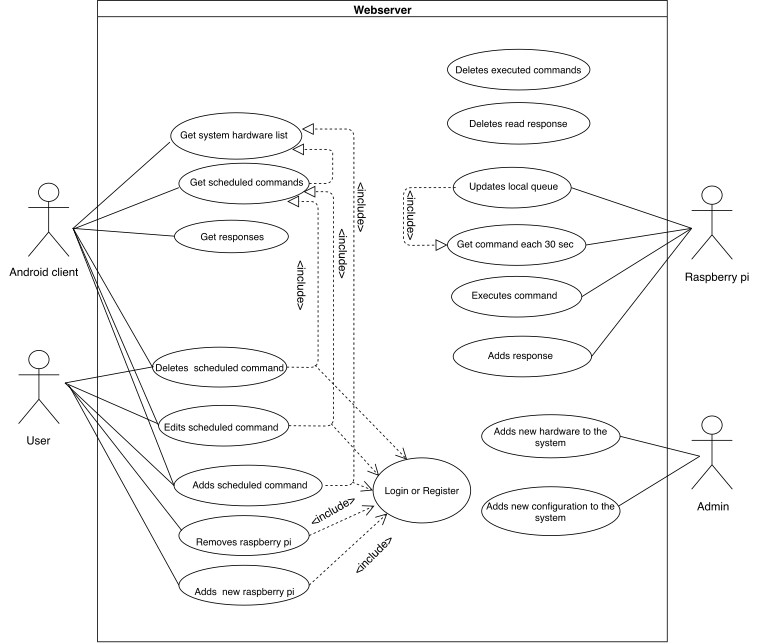
\includegraphics[width=\linewidth]{img/diagram_usecase.jpg}
					\end{figure}
				
				\newpage\subsubsection{Use Case Scenarios}
				
				\boldcolor{Android app gets hardware list}
				\newline\textbf{Goal:} to get all hardware in the system from webserver.
				\newline\textbf{Actors:} Android app, Web server.
				\newline\textbf{Precondition:} user opens android app.
				\newline\textbf{Primary Scenario:}	
				\begin{enumerate}[label*=\arabic*.]
					\item android app calls the webserver endpoint \code{/hardware}
					\item webserver fetches data from database using \code{hardware.index()}
					\item webserver responses to request with an array of hardwares in the response's body
					\item Android display this array to user in UI.
				\end{enumerate}
				\textbf{Variant:}\newline
				\hspace*{5mm}*. user might exist android app. \\
				\hspace*{5mm}1.android app might fail to connect to the internet \\
				\newline\boldcolor{Android app gets command list}
				\newline\textbf{Goal:} to get all commands in the system related to selected hardware.
				\newline\textbf{Actors:} Android app, Web server.
				\newline\textbf{Precondition:} android app gets hardware list
				\newline\textbf{Primary Scenario:}	
				\begin{enumerate}[label*=\arabic*.]
					\item user selects hardware from UI.
					\item android app calls the webserver endpoint \code{/hardware/\{hardwareId\}/command}, where \textit{hardwareId} is the id of the hardware the user selected.
					\item webserver fetches data from database using \code{command.indexByHardwareId(\{hardwareId\})}
					\item webserver responses to request with an array of commands in the response's body
					\item ando
				\end{enumerate}
				\textbf{Variant:}\newline
				\hspace*{5mm}*. user might exist android app. \\
				\hspace*{5mm}2.android app might fail to connect to the internet \\
				\newline\boldcolor{Raspberry pi executes commands}
				\newline\textbf{Goal:} to execute commands saved in the local queue on a timely fashion.
				\newline\textbf{Actors:} Raspberry Pi.	
				\newline\textbf{Precondition:} raspberry pi got the commands from webserver, updated local database.
				\newline\textbf{Primary Scenario:}	
				\begin{enumerate}[label*=\arabic*.]
					\item raspberry pi fetches first processed command saved in local queue.
					\item raspberry pi calls the function \code{EcecuteCommand()} and pass it the command as a parameter.
					\item raspberry pi look for the pin connecting the hardware and apply the desired configuration to it.
				\end{enumerate}
				\textbf{Variant:}\newline	
				\hspace*{5mm}1.a local queue might be empty, no action is taken. \\
				\hspace*{5mm}2.a a hardware error might happen, such as disconnected cable. \\
				\newline\boldcolor{Raspberry pi submits a command response to server}
				\newline\textbf{Goal:} to submit the result of the command execution to the server by saving it as a response row.
				\newline\textbf{Actors:} Raspberry Pi, webserver.
				\newline\textbf{Precondition:} raspberry pi executed commands.
				\newline\textbf{Primary Scenario:}	
				\begin{enumerate}[label*=\arabic*.]
					\item raspberry pi determines whether the execution was successful. 
					\item raspberry pi includes a message if any.
					\item  raspberry pi requests the webserver endpoint \code{/response} with the method \textit{POST}, needed parameter are added to the request body.
					\item webserver receives request, a new row to the database response table is added and ready for the android client to read. 
				 
				\end{enumerate}
				\textbf{Variant:}\newline	
				\hspace*{5mm}*. internet might disconnect.
					
						
				
				\newpage\subsubsection{Flowchart Diagram}
				% add webserver work, and change between webserver and web app
				\paragraph{} The flowchart for the system has three parallel processes: the raspberry pi process, the android app, and the android app back work.
				\begin{itemize}
					\item \boldcolor{Raspberry pi}: Every 30 seconds, raspberry first requests command list from the server, the web application then fetches the list from the database and returns it. Raspberry pi updates the local queue with them. It then checks the first command in the queue, if it was due it gets executed and post the response to the server. After execution, it checks the first in queue again.
					\item \boldcolor{Android app}: when android app is first opened, it requests hardware list from the webserver. After the web app fetches the hardware list from the database, it returns it to the android app, which displays the hardwares to the user. If the user clickes in a hardware, a new activity is opened containing the hardware information and the command list for that hardware. The user then can do 3 things: 
					\begin{enumerate}
						\item Edit a certain command: android request PUT to the command chosen from the server.
						\item Delete a certain command: android request DELETE to the command chosen from the server.
						\item Add a new command: android shows a new activity prompting the user for the command information, then it requests POST command to the server. 
					\end{enumerate}
					Regardless of the choice, the web app then process the request.
					\item \boldcolor{Android app back work}: each 5 or 10 minutes, android requests the responses from the webserver. When there is a response to be read, it shows it to the user as a push notification.
					\item \boldcolor{Web app}: when a command has no schedule and it was executed, the web app immediately deletes it from the database. Web app also deletes any read response.
				\end{itemize}
				\begin{figure}[H]
					\caption{Flow chart for the system}
					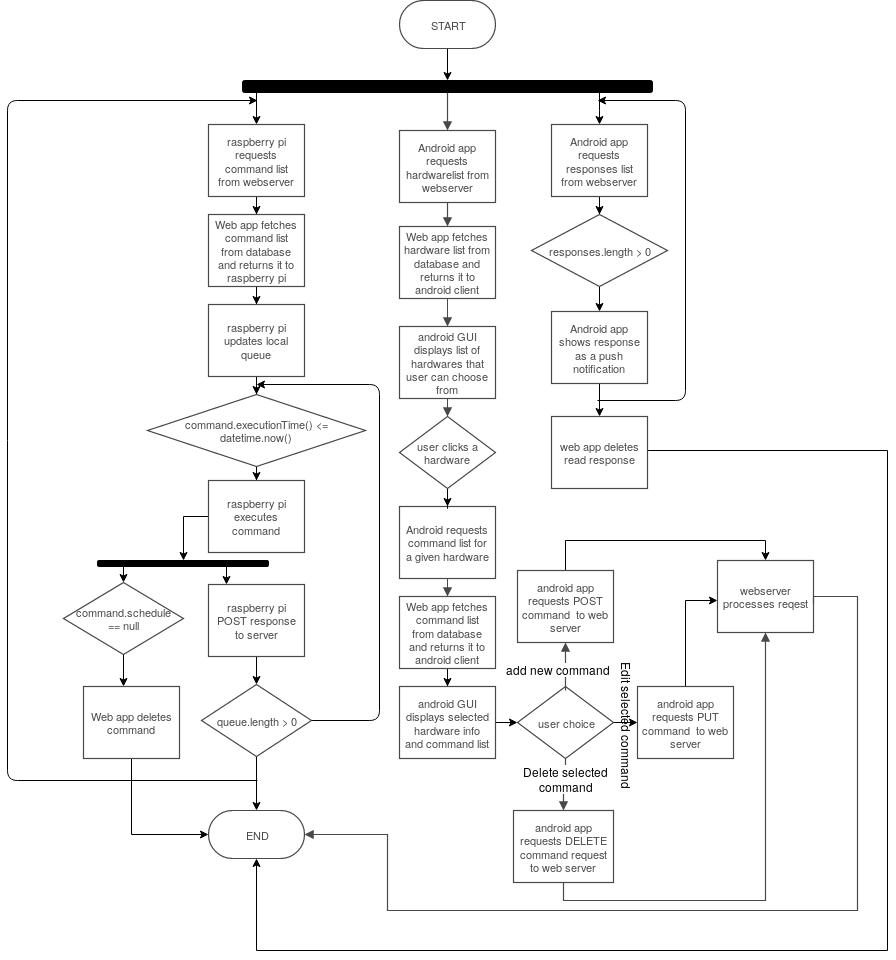
\includegraphics[width=\linewidth]{img/flowchart.png}
				\end{figure}
				\newpage\subsubsection{Entity Relationship Diagram}
					\paragraph{} In our system, there are two databases: the \textit{system database} stored in the web server, and \textit{the queue}, a local database for the raspberry pi. To make understanding the databases' easier, we represented it using entity relationship diagram. It is a graphical representation that demonstrates the relationship between concept, people, places, objects or events inside a system. The main components are the entities, relationship and cardinality. Entities are concepts or object that need their data stored. Cardinality defines that relationship in terms of numbers\cite{erd}.
				
				\begin{itemize}
					\item \boldcolor{System database}: This database is the main database. It will be stored in the web server and gets accessed by the android client and the raspberry pi. There are 5 main entities: 
					\begin{enumerate}
						\item \textbf{Hardware:} it will store information related to the physical components to raspberry pi. Such as LED lights, linear solenoid or an infra-red controller.  
						\item \textbf{Configuration:} hardwares can have different states. For example, a LED light could be on or off. An RGB LED can be ON on a certain color, of off. Configurations save the possible states a hardware can be in.
						\item \textbf{Command:} users can change raspberry pi's hardwares to be in a certain configuration. These commands are stored here. The users requests could either be instant, or scheduled. 
						\item \textbf{Schedule:} since commands can be scheduled, those data should be saved here. The user can choose the days and time a command fires.
						\item \textbf{Response:} when raspberry pi finish executing a command, it issues a response.
					\end{enumerate}
					\item \boldcolor{Local Queue}: This database is stored locally in raspberry pi. After raspberry gets user commands from server, it process them and order them based on their execution time.
					\begin{enumerate}
						\item \textbf{Hardware:} similar to the server's hardware list, this entity store the hardware connected. The system database gets data related to hardware from this entity 
						\item \textbf{Configuration:} this table stores the possible configuration. When the table is edited, the server database is updated.
						\item \textbf{PCommand:} only the commands to be executed are stored here, once a command is executed, it gets deleted from the queue. This entity contains processed commands. i.e each queue stores the exact date and time a command will be executed instead of the schedule information.
					\end{enumerate}
				\end{itemize}
			
			\textit{Figure \ref{fig:erd} shows the Entity-relationship diagram.} 
					\begin{figure}[H]
						\caption{Entity-relationship diagrams}
						\label{fig:erd}
						\begin{subfigure}[b]{\linewidth}
							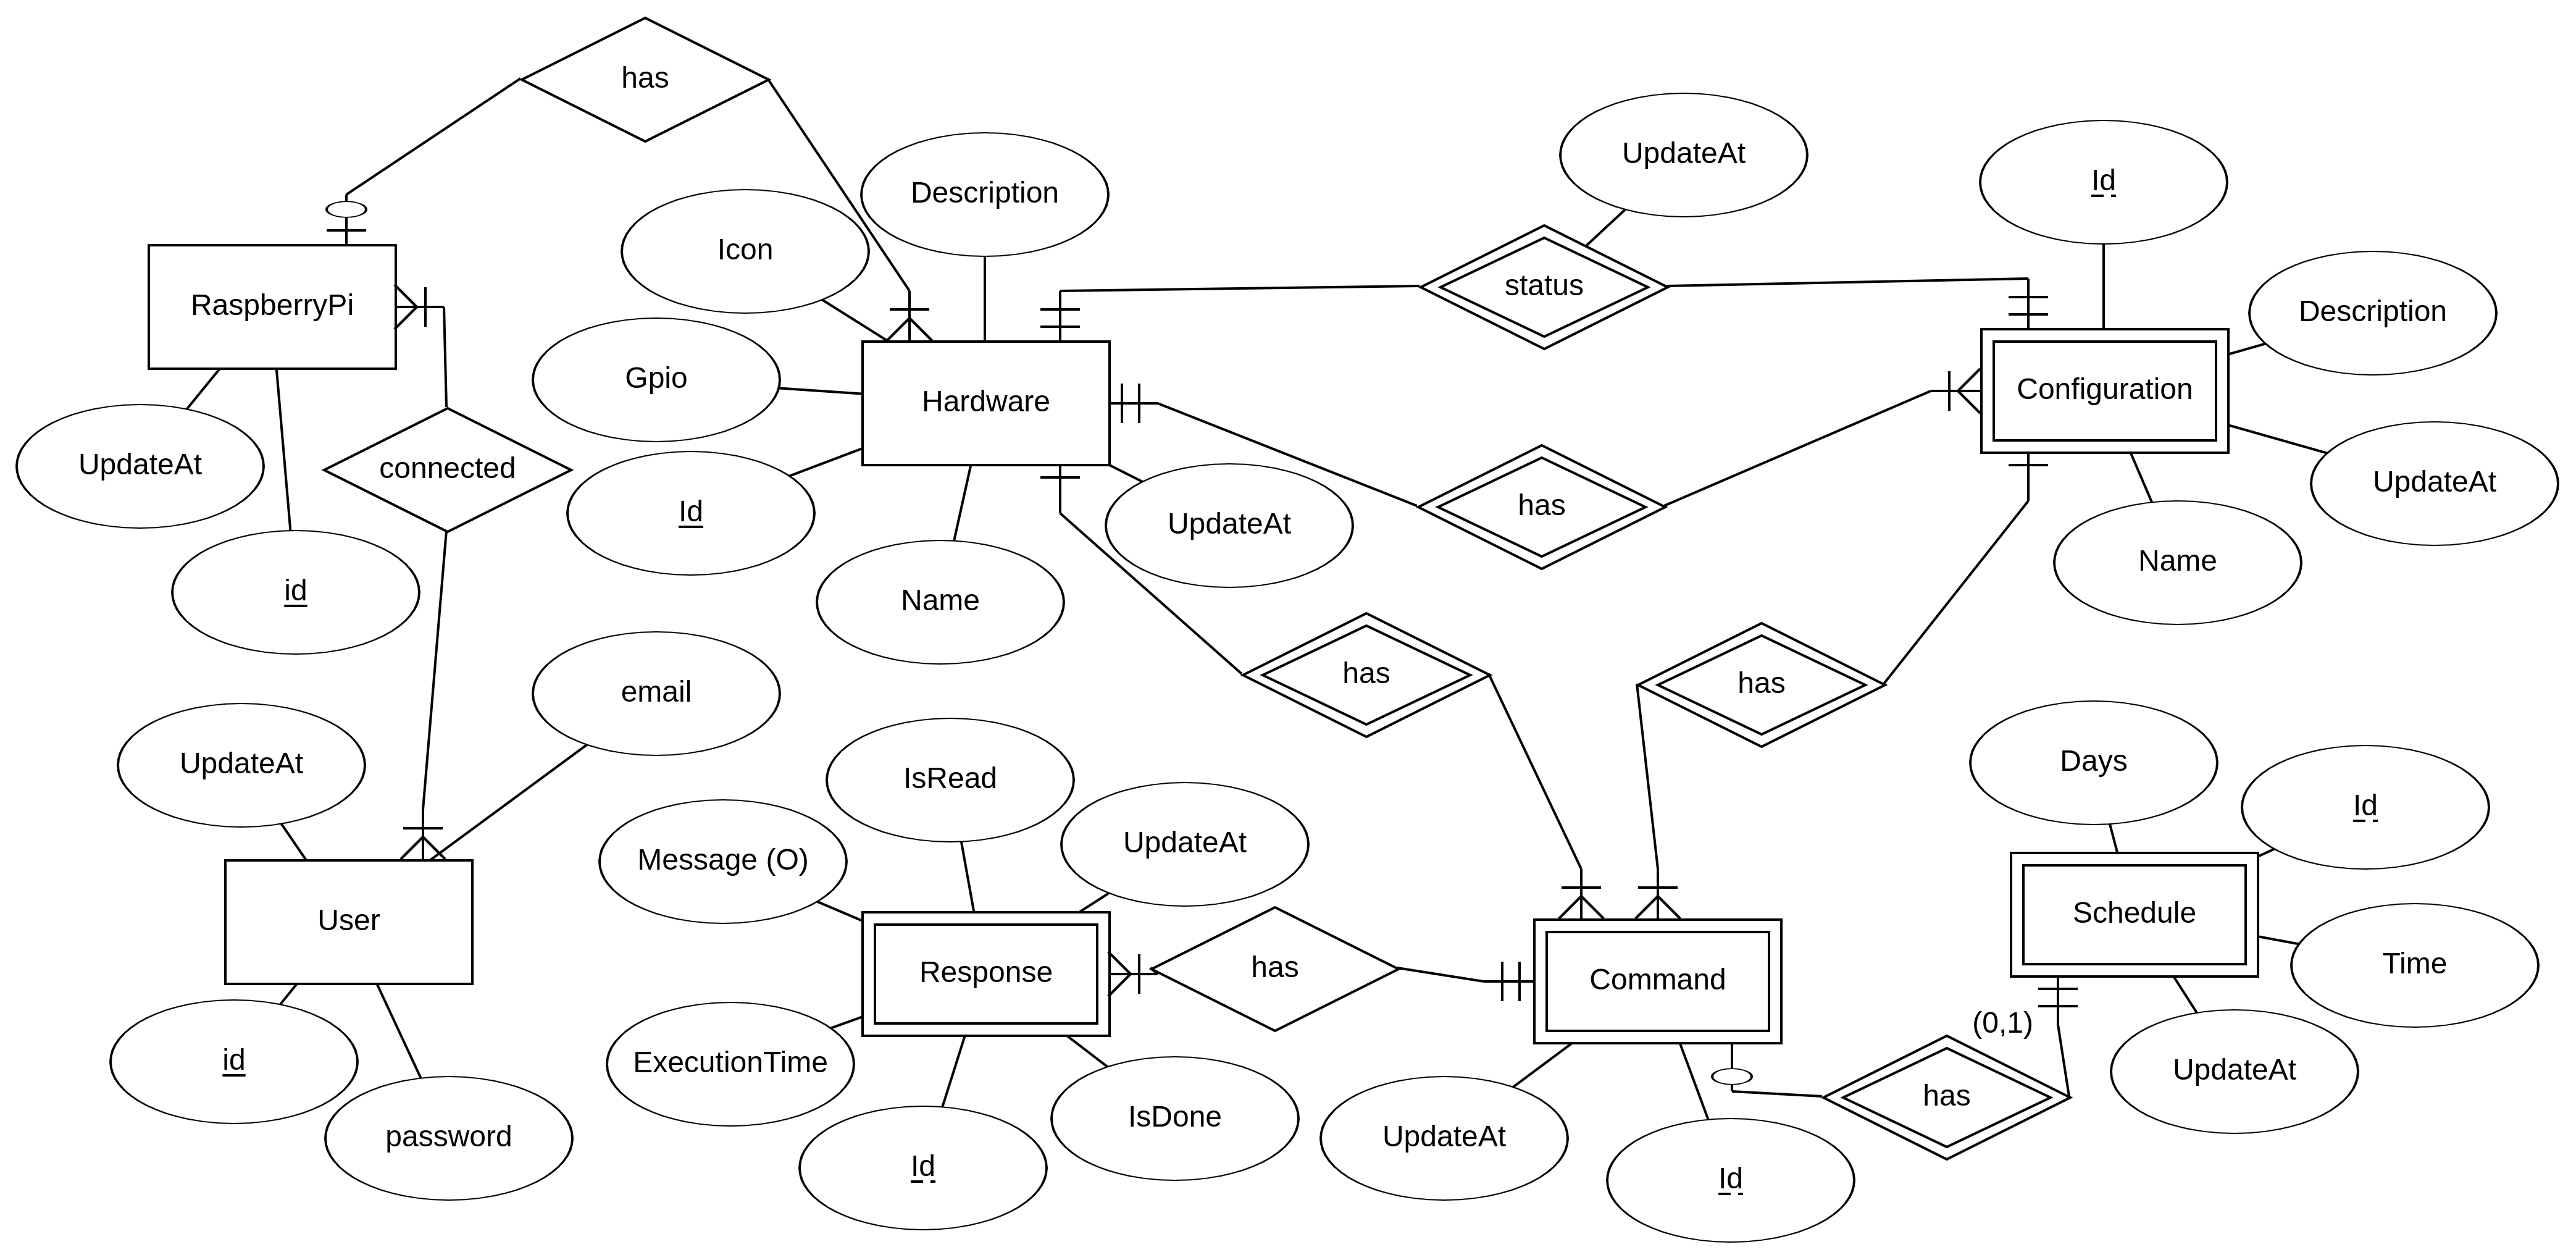
\includegraphics[width=\linewidth]{img/diagram_er1.png}
							\caption{System database}
						\end{subfigure}

						\begin{subfigure}[b]{\linewidth}
							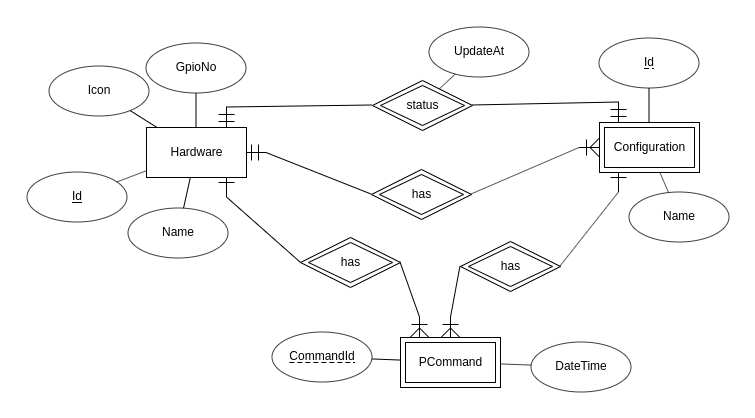
\includegraphics[width=\linewidth]{img/diagram_er2.png}
							\caption{Local queue}
						\end{subfigure}
					\end{figure}
				
			\newpage\subsection{Object-Oriented Diagrams}
				\subsubsection{Sequence Diagrams}
				\begin{figure}[H]
					\caption{Raspberry pi executes commands}
					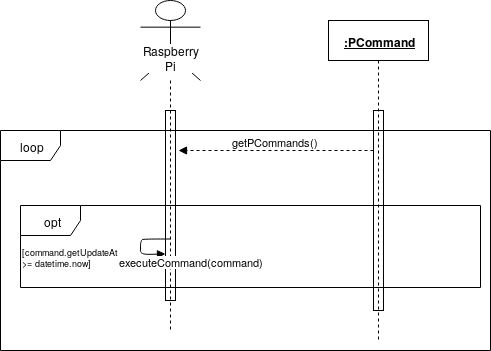
\includegraphics[width=\linewidth]{img/sequence_execute.png}
				\end{figure}
				\begin{figure}[H]
					\caption{Raspberry pi submits a command response to server}
					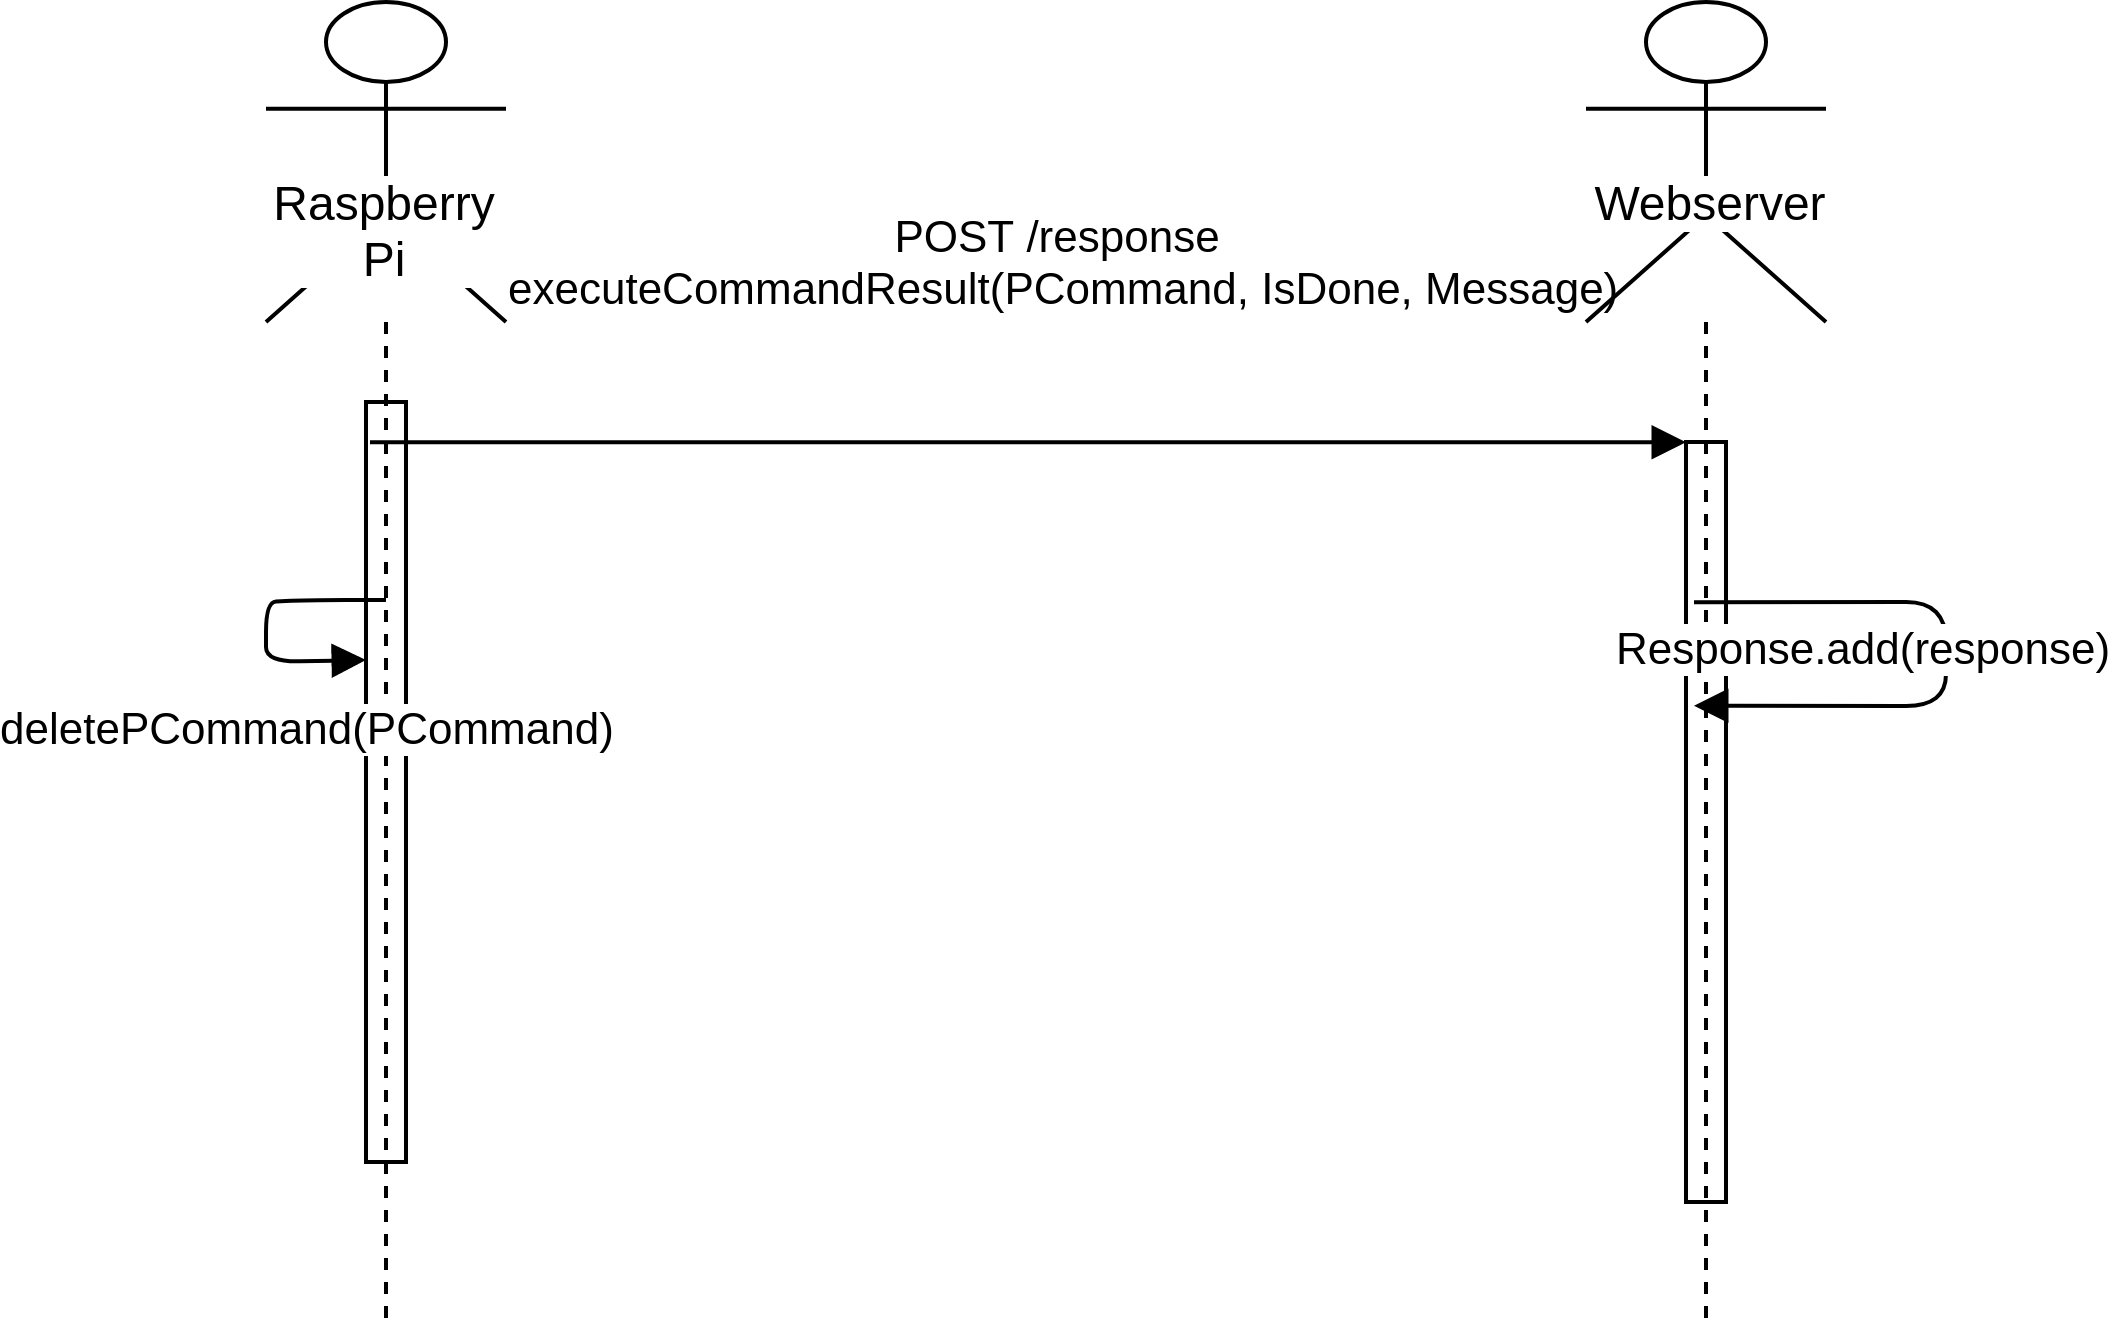
\includegraphics[width=\linewidth]{img/sequence_submit_response.png}
				\end{figure}
				\newpage\subsubsection{Class Diagram}
					\paragraph{} \textit{Figure \ref{fig:class_web}} shows the class diagram for the web application, and \textit{figure \ref{fig:class_rp}} shows the class diagram for raspberry pi.The classes are essentially wrappers for the databases tables, except for the class \textbf{RaspberryPi}, where the functions for controlling the hardwares are.
					\paragraph{}The classes which represent database's tables inherit from a \textbf{BaseEntity} generic class. This generic class has the entity's id and \textbf{updateAt} property, which determines when the entity was created/last updated. This generic class is important as it has the methods needed to communicate with the web server. An example is \code{hardware.edit(1)}, which corresponds to the REST API \textbf{PUT} \code{/hardware/1}.
					\begin{figure}[H]
						\caption{Class diagram for the web application}
						\label{fig:class_web}
						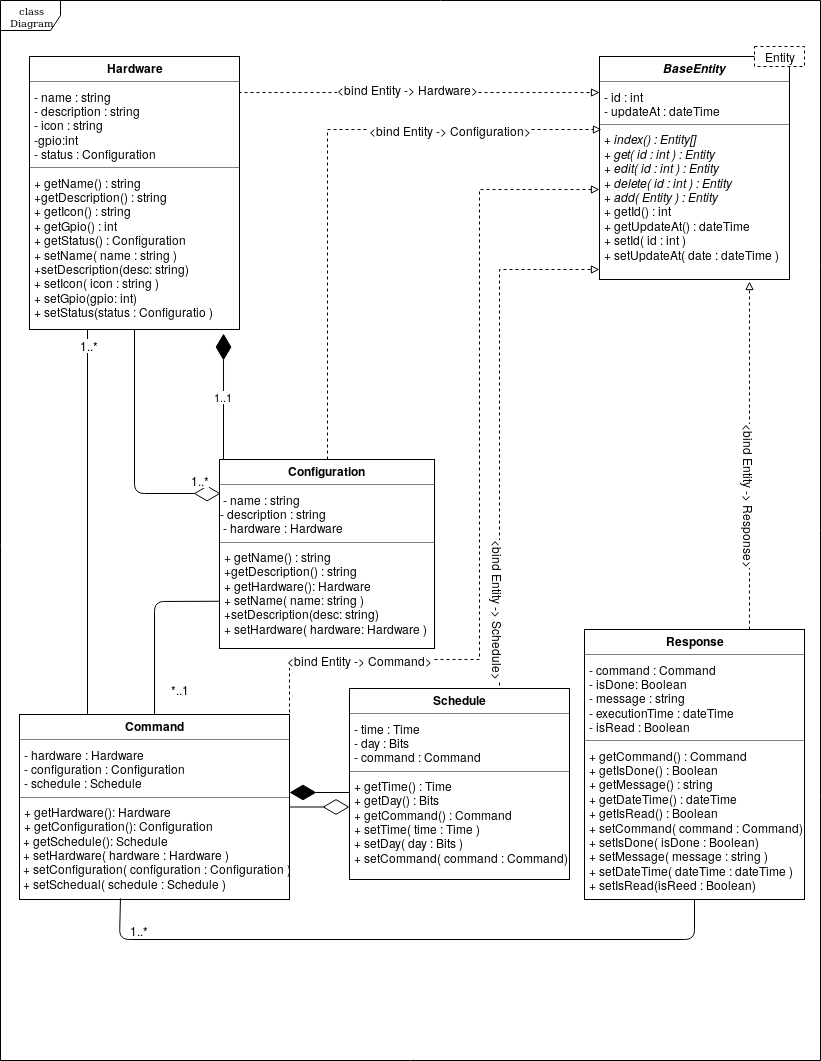
\includegraphics[width=\linewidth]{img/diagram_class1.png}
					\end{figure}
					\begin{figure}[H]
						\caption{Class diagram for the raspberry pi}
						\label{fig:class_rp}
						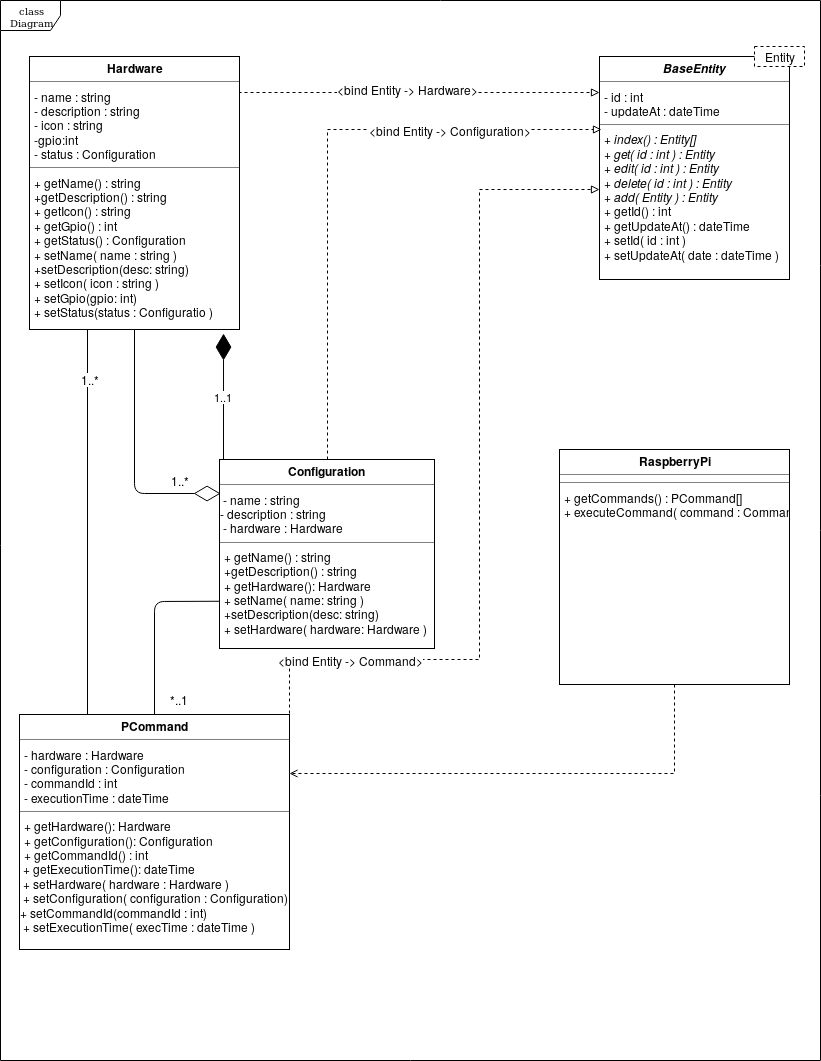
\includegraphics[width=\linewidth]{img/diagram_class2.png}
					\end{figure}
				\newpage\subsubsection{UML representation of the REST API Diagram}
				\paragraph{} Correct calls to the web application via the REST API is the building block of our project. Thus, talking about the structure is essential. The API has 5 entities representing the database's tables. For each entity, client can use 2 methods with the entity url -e.g. \code{/hardware}-: 
				\begin{itemize}
					\item \textbf{GET}: this method corresponds to the SQL's \code{SELECT * from ...;}.
					\item \textbf{POST}: a body of type JSON is required. It holds the object attributes. This method corresponds to the SQL's \code{INSERT INTO}.
				\end{itemize} 
			 	\paragraph{}Also, client can use 3 methods with the entity url + id -e.g.\code{/hardware/6}-: 
			 	\begin{itemize}
			 		\item \textbf{GET}: this method corresponds to the SQL's \code{SELECT * from ... WHERE id = ...;}.
			 		\item \textbf{PUT}: a body of type JSON is required. It holds the object attributes. This method corresponds to the SQL's \code{UPDATE ... WHERE id = ..;}.
			 		\item \textbf{DELETE}: this method corresponds to the SQL's \code{DELETE FROM ... WHERE id = ..;}.
			 	\end{itemize} 
		 		\textit{Figure \ref{fig:rest} shows the API's hierarchy and figure \ref{fig:rest_model} shows the models. For full documentation see Appendix \ref{appendix:api_doc}}
				\begin{figure}[H]
					\caption{REST API}
					\label{fig:rest}
					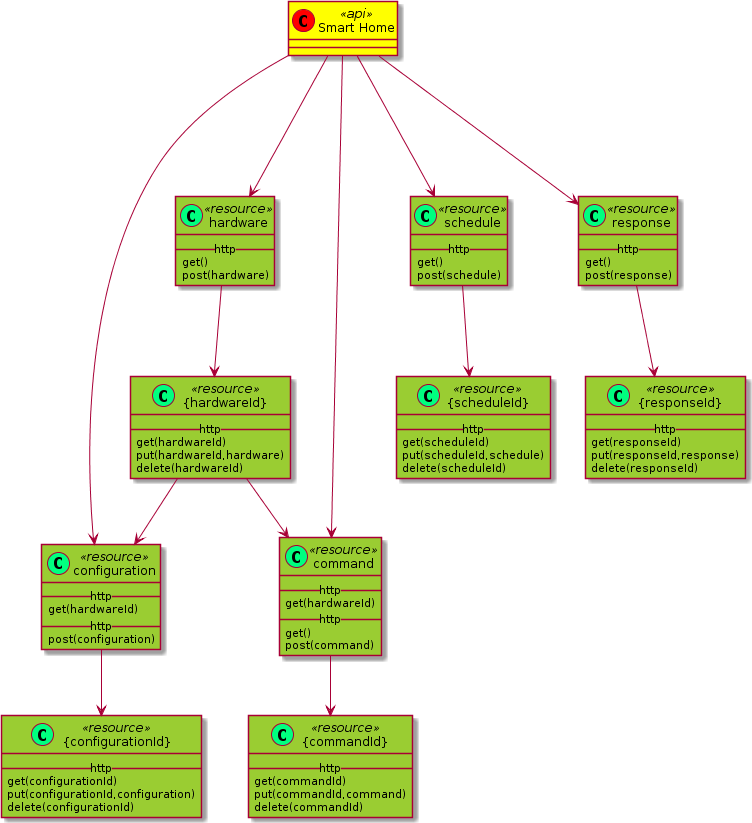
\includegraphics[width=\linewidth]{img/rest_uml.png}
				\end{figure}
			\begin{figure}[H]
				\caption{REST API models}
				\label{fig:rest_model}
				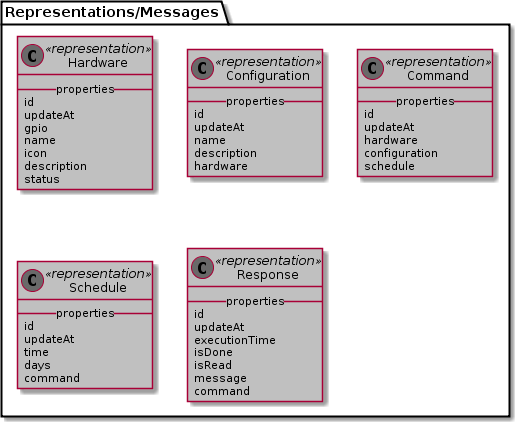
\includegraphics[width=\linewidth]{img/rest_uml_model.png}
			\end{figure}	
		\newpage
	\begin{comment}
		usecase
		sequence
		desc
		
		ERD
			
	\chapter{System Design}
		\section{System Architecture}
		\section{User Interface Design}
		\newpage	
	\chapter{Implementation}
		\section{Implementation}
		\section{Implementation Requirements}
			\subsection{Software Requirements}
			\subsection{Hardware Requirements}
		\section{Implementation Detailed}
		\section{I/O Screens}
		\newpage	
	\chapter{Testing}
		\section{Testing}
		\section{Test Plan}
			\subsection{Unit Test}
			\subsection{Functional Test}
			\subsection{Acceptance Test}
		\section{Test Items}
			\subsection{Features to Be Tested}
			\subsection{Schedule of Test Actions}
			\subsection{Test Tasks}
		\section{Test Case}
		\section{Test Result}
		\newpage	
	\chapter{Conclusion}
		\section{Conclusion}
		\section{Evaluation}
		\section{Future Work}
	\newpage
	
	
	
	\end{comment}
	\bibliographystyle{ieeetr}
	\renewcommand{\bibname}{References}
	\bibliography{References}


	\clearpage
	\mychapter{Appendices}
	\appendix
	%\renewcommand{thesection}{\Alph{section}}
		\chapter{Figures}
		\label{appendix:similar_system_comparision}
		\section{Similar systems hub design}
		\begin{figure}[H]
			\caption{Similar systems: hub design}
			\begin{subfigure}[b]{.5\linewidth}
				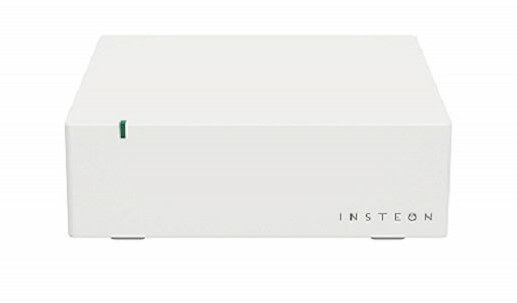
\includegraphics[width=\linewidth]{img/insteon_hw.png}
				\caption{Insteon}
			\end{subfigure}
			\begin{subfigure}[b]{.5\linewidth}
				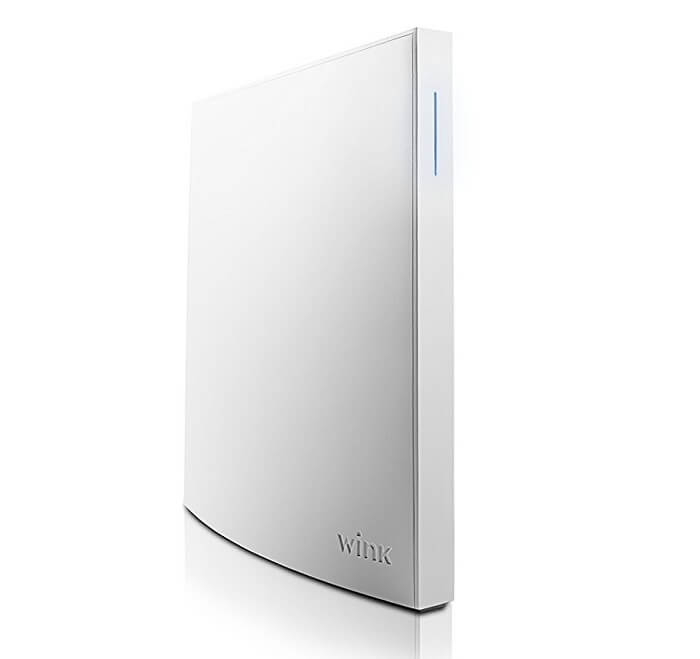
\includegraphics[width=\linewidth]{img/wink_hw.png}
				\caption{Wink}
			\end{subfigure}
			\begin{subfigure}[b]{.5\linewidth}
			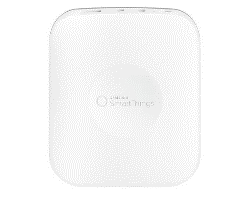
\includegraphics[width=\linewidth]{img/samsung_hw.png}
				\caption{Samsung}
			\end{subfigure}
			\begin{subfigure}[b]{.5\linewidth}
				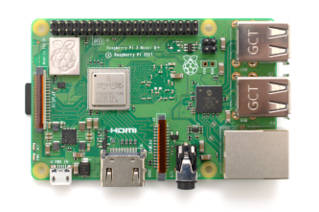
\includegraphics[width=\linewidth]{img/raspberry.png}
				\caption{Raspberry Pi}
			\end{subfigure}
		\end{figure}

		\newpage\chapter{REST API Documentation}
		\label{appendix:api_doc}
		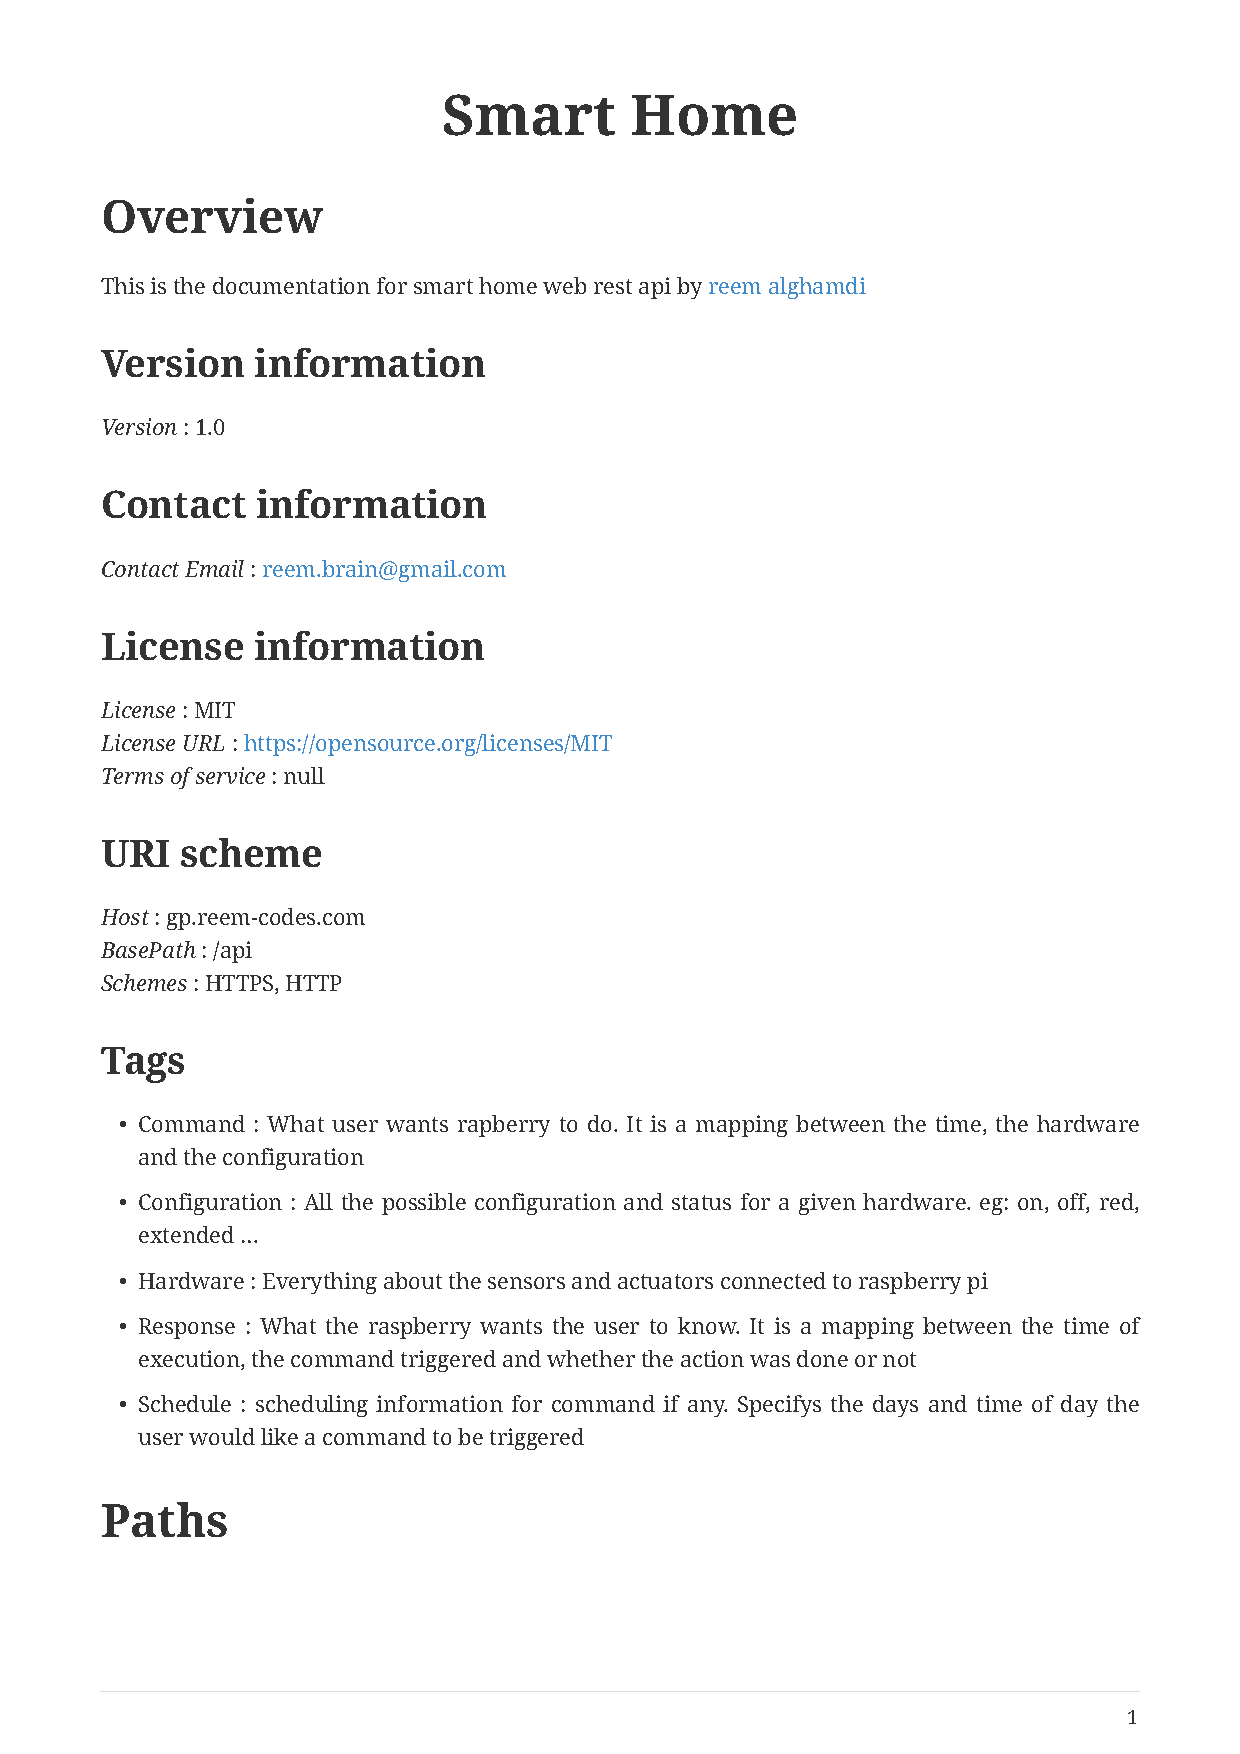
\includepdf[pages=-, width=\linewidth, pagecommand={\pagestyle{fancy}}]{file/api-documentation.pdf}

\end{document}


	\begin{comment}
	TODO:
	# nouf IoT
	# Doha class
	
	
	# muna flow chart
	# Doha data flow
	# all functions
	# REST API Swagger
	\end{comment}
